
\chapter{Context-Aware Speculative Decoding}
\label{sec:casd}

There are many stand-alone techniques to do speculative decoding. Each technique tries to perform as good as it can by itself. However, what seems to be underexplored in the domain of speculative decoding is the possibility of augmenting techniques. An augmenting technique will use a strong baseline method and try to fill in the gaps, where the baseline model underperforms. This principle is shown in Figure \ref{fig:spec_dec_casd_augment}. To have a good augmenting model, it must be fundamentally different from the baseline model. We present Context-Aware Speculative Decoding (CASD), which is such an augmenting technique, that generates drafts where the current SOTA (EAGLE-2 \cite{li2024eagle}) underperforms.

\begin{figure}[h]
	\centering
	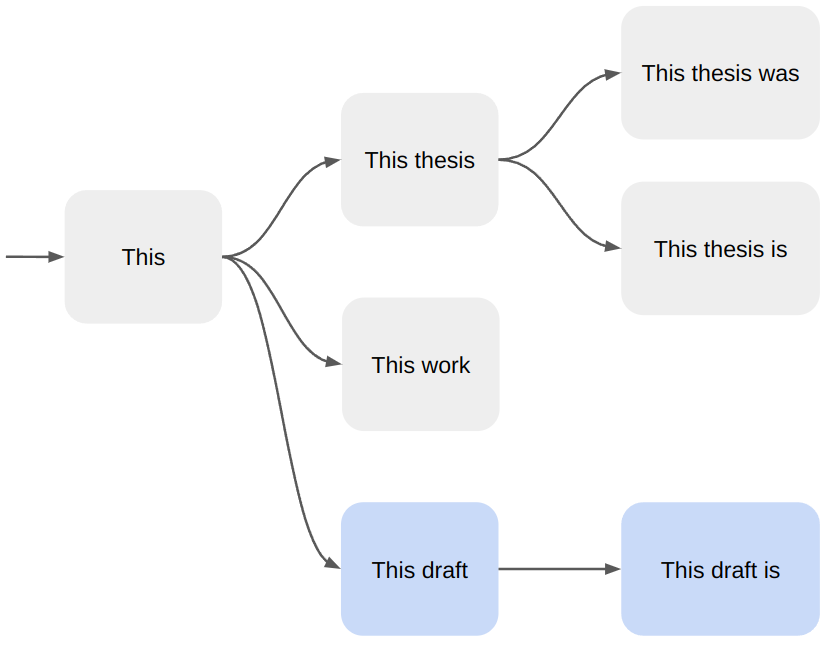
\includegraphics[width=0.7\linewidth]{fig/spec_dec_casd_augment.png}
	\caption{An example draft by a \textcolor{darkgray}{base speculator} (e.g. EAGLE-2) and an \textcolor{blue-ish}{augmenting method} (e.g. CASD). The augmenting method has merged its drafts with the baseline's drafts to form one draft tree.}
	\label{fig:spec_dec_casd_augment}
\end{figure}

\section{Research hypothesis}
A common use case for LLMs is to use it in a RAG framework. As Section \ref{sec:rag} explains, RAG uses an LLM to answer questions based on some relevant document chunks, so the context of the LLM is prefilled with chunks before answering. This context contains the facts that the LLM is expected to use in its answer. To improve factuality, the preprompt often contains explicit or implicit instructions to use or even copy the context. This is what Context-Aware Speculative Decoding will try to pick up on. When the LLM will copy long sequences of tokens from the context, a reasonable draft could be made by just looking at the context. The hypothesis is that this yields long, good drafts, that are quite independent from neural-based methods.

\section{Drafting method of CASD}
CASD is a lightweight statistical method to generate speculative samples from the context itself. To do so, the last generated tokens are searched in the full context, as shown in Figure \ref{fig:CASD_example_prompt}. If at least one token corresponds to the last generated tokens, we call it a match. When there are multiple matches found in the context, the top 2 are kept based on how long the match was. Then, up to 10 tokens after the match are copied as drafts. Finally, the drafts are merged with those of EAGLE-2.

\begin{figure}[h]
	\centering
	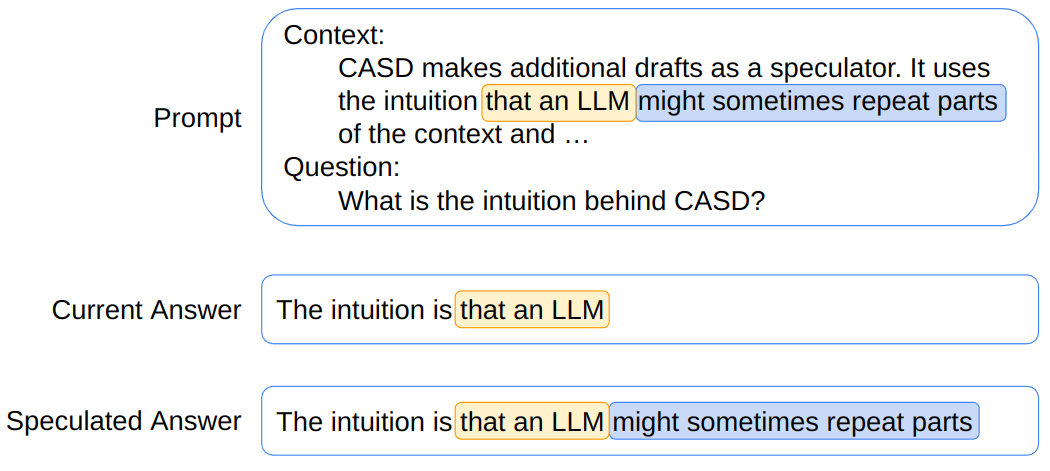
\includegraphics[width=0.7\linewidth]{fig/CASD_example_prompt.png}
	\caption{CASD applied to a simplified RAG prompt. The \textcolor{orange-ish}{prefix} (``that an LLM'') is found in the context and thus the \textcolor{blue-ish}{continuation} (``might sometimes repeat parts'') is drafted by CASD.}
	\label{fig:CASD_example_prompt}
\end{figure}

\section{Results}
In this section, we analyze the performance of CASD, mainly comparing with EAGLE-2.

\subsection{Experimental setup}
\textbf{Models.} The experiments use only Llama-3-8B-Instruct \cite{grattafiori2024llama} as an LLM, as only this model fits our following constraints. The first constraint is the hardware: 8B is the largest model that fits on the used GPU. Since one of our benchmarks has Dutch content (UZGentRAG, see further), we also need a Dutch-capable LLM. Lastly, the SOTA baseline, EAGLE-2 also has to support the LLM. This yields Llama-3-8B-Instruct as the chosen model for all experiments. 

\textbf{Tasks.} CASD is evaluated on our private UZGentRAG benchmark (see further), SQuAD \cite{rajpurkar2016squad} and the classical speculative decoding benchmarks (Alpaca \cite{alpaca}, GSM8K \cite{cobbe2021gsm8k}, HumanEval \cite{chen2021evaluating}, MT-bench \cite{zheng2023judging}, Natural Questions a.k.a. QA \cite{kwiatkowski2019natural} and CNN/DM \cite{nallapati2016abstractive}). All experiments were performed with batch size 1, conform with most related work \cite{kim2023speculative, leviathan2023fast, li2024eagle, zhou2023distillspec}.

\textbf{Metrics.} CASD, being an augmenting method, focuses on improvements on the baseline speculator. The usual speculative decoding metrics, applied to CASD are:
\begin{itemize}
  \item \emph{Walltime speedup ratio}: The speedup ratio relative to the baseline method, EAGLE-2.
  \item \emph{Average acceptance length} $\tau$ : The average number of tokens accepted per forward pass of the target LLM.
  \item \emph{Energy improvement}: The improvement in energy efficiency relative to the baseline method.
\end{itemize}

We approximate the energy consumption by the consumption of the GPU only. This is because our virtualized setup could not measure CPU and RAM energy accurately. However, the energy consumption of the whole system is primarily determined by the GPU \cite{li2024unseen}, so this indicator should be reasonably accurate.

\subsection{UZGentRAG benchmark}
We hypothesized that EAGLE-2 would underperform in multilingual settings and niche domains. This is because EAGLE-2 is trained on mostly English data in rather general domains (ShareGPT \cite{shareGPT}). That means niche domains are out-of-distribution and neural networks are known to have bad performance on out-of-distribution input. We must note that the neural network of EAGLE-2 works on top of the features of the LLM, so if the LLM is trained to have language-agnostic features that would not be the case. However, the latest LLMs are typically not trained in that way and thus the problem remains.

To prove our hypothesis, we had to go beyond the standard English speculative decoding benchmarks. However, low-resource languages such as Dutch have limited benchmarks available and for RAG use cases we did not find any. That is why we made our own benchmark. As mentioned in Section \ref{sec:uzgent_test_results_and_feedback}, we held a test session at UZGent. In that session, we not only evaluated the RAG system, but we also constructed UZGentRAG, a private niche RAG benchmark in Dutch and for the medical domain. This benchmark contains the queries logged from the daily work of doctors and nurses, by recording their questions to a chatbot. Internal UZGent documents found by the chatbot were combined with the query in a typical RAG prompt. These prompts form the benchmark, as that is the only data necessary to test a speculative decoding method.

While we cannot make the entire dataset public, we are allowed to give some insights. Table \ref{tab:uzgentrag_benchmark} shows some relevant statistics of UZGentRAG, compared with SQuAD. The number of prompts of UZGentRAG is rather limited for a benchmark, however we see that EAGLE-2 uses 80 questions per benchmark and for speculative decoding that order of magnitude seems acceptable. That is also the reason our RAG adaptation of SQuAD was capped at 80 questions. The prompt length might also surprise, because SQuAD has rather large prompts. This is because the adaptation required few-shot prompting to achieve satisfactory answers from the LLM and those few shots take up some space in every prompt. For the length in tokens, we used the Llama 3 \cite{grattafiori2024llama} tokenizer, consistent with our experiments later. The last metric, BLEU, is good at measuring how much is copied between context and answer; exactly what CASD needs. It is clear that UZGentRAG often requires copying from the context, but that holds even more for SQuAD. As this thesis is not about the BLEU score, we do not further elaborate on how this metric checks for copying. For reproducibility, it needs to be said that we edited the metric to have no brevity penalty as this is not relevant to our use case.

\begin{table}[h]
    \centering
    \begin{tabular}{l|cc}
         & UZGentRAG & SQuAD (RAG) \\
        \hline
        language & Dutch & English \\
        \# prompts & 165 & 80 \\
        \# chunks per prompt & 3 & 1 \\ 
        mean prompt length & 2420 char - 780 tokens & 2947 char - 615 tokens\\
        mean answer length & 849 char - 83 tokens & 83 char - 18 tokens\\
        %BLEU score & 0.06 & 0.0000003\\
        BLEU score (no brevity penalty) & 0.25 & 0.64\\
    \end{tabular}
    \caption{Statistics of UZGentRAG benchmark, compared with the most similar benchmark: SQuAD (adapted for RAG with speculative decoding).}
    \label{tab:uzgentrag_benchmark}
\end{table}

In order to give some idea what a typical UZGentRAG prompt might look like, one shortened example is given below. For the full prompt, we refer to Appendix \ref{sec:example_prompt}.

\begin{wrapverbatim}
[begin context]
Jij bent een dokter. Jij kent alle medische procedures van het UZGent.
[einde context]
[begin documenten]
*chunk 1*
---
*chunk 2*
---
*chunk 3*
[einde documenten]
[begin vraag]
Wat moet ik doen bij een graad 1 immuun-gerelateerde hypothyroïdie?
[einde vraag]
[begin antwoord]

\end{wrapverbatim}


\subsection{Performance of CASD}
\begin{figure}[h]
  \centering
  \captionsetup{justification=centering}
  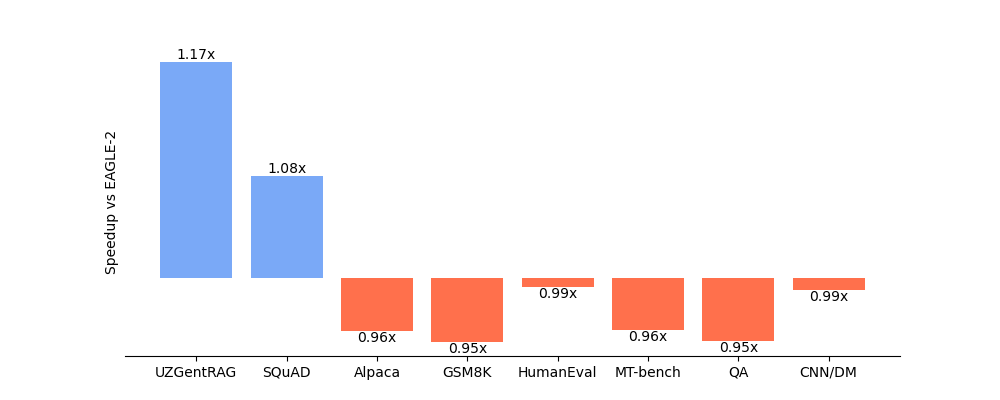
\includegraphics[width=\linewidth]{fig/speedup_vs_eagle.png}
  \caption{Speedup of CASD compared to the baseline, EAGLE-2. CASD yields improvements for both RAG benchmarks. On standard speculative decoding benchmarks the overhead is still rather limited.}
  \label{fig:speedup_vs_eagle}
\end{figure}

Figure \ref{fig:speedup_vs_eagle} shows the comparison between CASD and EAGLE-2. The most relevant benchmarks are the RAG benchmarks, UZGentRAG and SQuAD, for which CASD achieved a speedup of 1.17 and 1.08 respectively. This is quite interesting, because both benchmarks are RAG use cases, yet the results differ strongly. We hypothesize that the Dutch UZGentRAG is harder for EAGLE-2, so it is easier for CASD to find better continuations.

Next to the RAG benchmarks, we also list the general benchmarks. Since these are not RAG-based, and EAGLE-2 was designed for these settings, performance is now greater for EAGLE-2. The key takeaway here is that even when applying CASD to non-RAG input, it still has limited overhead (1-5\%).

The full details of the performance can be seen in Table \ref{tab:performance_benchmarks}. The first thing that stands out is that the relative increase of the number of correctly speculated tokens ($\tau_{CASD} / \tau_{EAGLE-2}$) is higher for SQuAD than for UZGentRAG. In other words, the number of LLM calls were reduced most for SQuAD and nevertheless the speedup is much higher for UZGentRAG. This likely means that SQuAD had many more substring matches, increasing the overhead of CASD and thus slowing down the total system.

Another interesting deduction we can make is that UZGentRAG successfully addresses the pain points of EAGLE-2. It has a $\tau$ of around 4 in general use cases, around 6 in the case of SQuAD (RAG) and only 2.09 for UZGentRAG (also RAG). This strong difference shows that EAGLE-2 struggles with the combination of Dutch and the medical domain. The scope of this thesis did not allow a further study to see whether Dutch or the medical domain was the dominating factor here.

\begin{table}[h]
    \centering
    \begin{tabular}{cccc|cc|cc}
        & & \multicolumn{2}{c}{CASD} & \multicolumn{2}{c}{EAGLE-2} & \multicolumn{2}{c}{CASD vs EAGLE-2} \\
        \cline{3-8}
        & & Tokens/s & $\tau$ & Tokens/s & $\tau$ & Speedup & $\tau_{CASD} / \tau_{EAGLE-2}$ \\
        \hline
        \multirow{2}{*}{RAG benchmarks} & UZGentRAG & \textbf{35} & \textbf{2.73} & 30 & 2.09 & 1.17 & 1.30 \\
        & SQuAD             & \textbf{46} & \textbf{7.78} & 43 & 5.88 & 1.08 & 1.32 \\
        \hline
        \multirow{6}{*}{General benchmarks} & Alpaca & 61 & \textbf{4.15} & \textbf{64} & 4.12 & 0.96 & 1.01 \\
        & GSM8K             & 64 & \textbf{4.56} & \textbf{67} & 4.42 & 0.95 & 1.03 \\
        & HumanEval         & 75 & \textbf{5.55} & \textbf{76} & 5.05 & 0.99 & 1.10 \\
        & MT-bench          & 61 & \textbf{4.35} & \textbf{63} & 4.18 & 0.96 & 1.04 \\
        & QA                & 52 & \textbf{3.56} & \textbf{54} & 3.53 & 0.95 & 1.01 \\
        & CNN/DM            & 52 & \textbf{4.14} & \textbf{52} & 3.74 & 0.99 & 1.11 \\
        \hline
    \end{tabular}
    \caption{Performance of CASD compared with the baseline EAGLE-2. The best score is in bold.}
    \label{tab:performance_benchmarks}
\end{table}

\subsection{Energy improvements by CASD}
\begin{figure}[h]
  \centering
  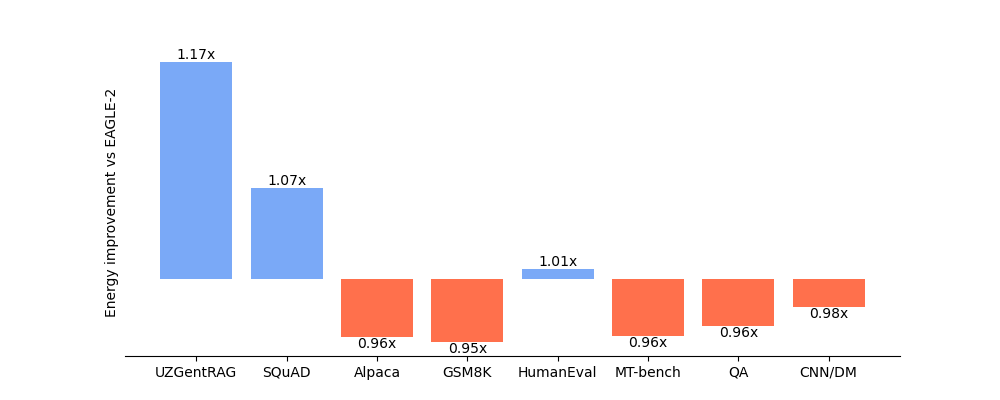
\includegraphics[width=\linewidth]{fig/energy_vs_eagle.png}
  \caption{GPU Energy improvements of CASD compared to the baseline, EAGLE-2. CASD yields improvements for both RAG benchmarks. On standard speculative decoding benchmarks the overhead is again rather limited.}
  \label{fig:energy_vs_eagle}
\end{figure}

Figure \ref{fig:energy_vs_eagle} shows the improvement in GPU energy consumption. Interestingly, we see very similar numbers as for the speedups. This should not necessarily be the case and it depends on the speculator's speed-efficiency, power-efficiency and token-efficiency, so it is a pure coincidence. Practically, this means the conclusions are the same: applying CASD to RAG use cases yields improvements and applying it to other cases generally yields worse results. As a side note, HumanEval did see a slowdown of 1\%, but also an energy improvement by 1\%, making it the only benchmark that has opposite results. However, the difference is insignificant and might as well be noise on the measurements.

\subsection{Acceptance length}
\begin{figure}[h]
  \centering
  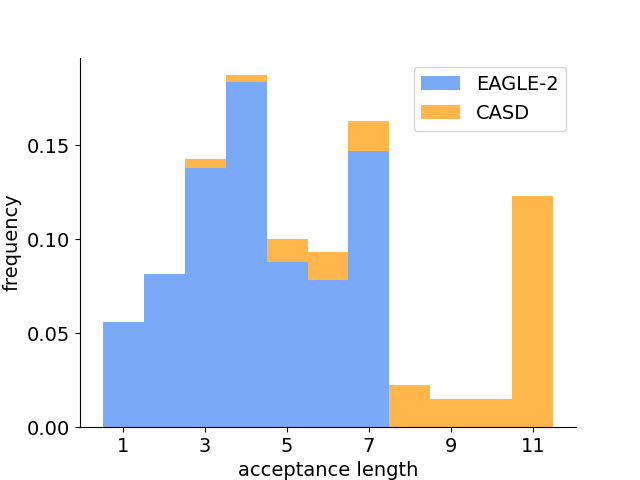
\includegraphics[width=0.7\linewidth]{fig/acceptance_length.png}
  \caption{Distribution of acceptance lengths with CASD augmenting EAGLE-2. CASD supplements EAGLE-2 with long-length drafts.}
  \label{fig:acceptance_length}
\end{figure}

To understand why CASD yields improvements on neural speculators, Figure \ref{fig:acceptance_length} shows how the acceptance length is distributed. EAGLE-2 works quite well and rather consistently: most often it has 4 to 7 tokens accepted. On the other hand, CASD's added speculations show a strong peak at 11. So if CASD gives the best speculation, it is a high quality speculation for a long length. This also explains intuitively why CASD works so well with neural speculators: CASD has occasional speculations that are extremely good, while the neural speculator works well consistently when nothing is copied. As a last remark, it might stand out that there is a hard cap at 7 and 11 for EAGLE-2 and CASD respectively. Both methods implement this cap to balance overhead with more accepted tokens.

\subsection{Ablation study}

CASD copies drafts from the entire context, but also from the tokens that were already generated. However, for the original problem statement (RAG), CASD only had to copy from the prompt and not from the answer that the LLM had generated up until that point. If CASD did that, it could be better if the LLM almost never copies from the generated tokens, as it has a smaller overhead. The opposite could as well be true, where CASD benefits now from an LLM repeating itself. The following empirical tests show whether the extra LLM tokens actually provide benefits: we compare our original CASD to CASD$_{prompt}$, which only considers prompt tokens.

Table \ref{tab:ablation_benchmarks} shows how CASD$_{prompt}$ performs. For the most relevant benchmark, UZGentRAG, a slight improvement justifies the choice of CASD over CASD$_{prompt}$. For SQuAD, $\tau$ stayed the same and so did the throughput. Finally, MT-bench shows very similar performance. So it seems that CASD performs better than CASD$_{prompt}$, mostly on the UZGentRAG benchmark. As this benchmark contains longer answers than SQuAD, we intuitively think that the LLM starts repeating generated fragments more the longer the answer gets.

\begin{table*}[h]
  \centering
  \begin{tabular}{ccc|cc|cc}
      & \multicolumn{2}{c}{CASD} & \multicolumn{2}{c}{CASD$_{prompt}$} & \multicolumn{2}{c}{EAGLE-2} \\
      \cline{2-7}
      & Tokens/s & $\tau$ & Tokens/s & $\tau$ & Tokens/s & $\tau$ \\
      \hline
      UZGentRAG & \textbf{35} & \textbf{2.73} & 34 & 2.65 & 30 & 2.09 \\
      SQuAD     & \textbf{46} & \textbf{7.78} & \textbf{46} & \textbf{7.78} & 43 & 5.88 \\
      MT-bench  & 61 & \textbf{4.35} & 61 & 4.30 & \textbf{63} & 4.18 \\
      \hline
  \end{tabular}
  \caption{Performance of CASD$_{prompt}$ compared to CASD and EAGLE-2 as the baseline. The best score is indicated in bold.}
  \label{tab:ablation_benchmarks}
\end{table*}

\section{Further analysis}
\label{sec:further_analysis}
This section shows the reasoning behind some implementation choices, by further analyzing CASD.

In CASD, we only take the top-2 matches according to match length. This implicitly assumes that longer matches are better and Figure \ref{fig:prob_casd_accept} (a) validates this assumption. The first interesting feature is that the further to the right, the higher the probability (typically), and this for all rows. This shows that the average accepted length grows longer with longer match lengths. But not only does this validate that longer matches generate better speculations, it also opens up an area of future work. Instead of taking the 10 next tokens of a match regardless of the match length, CASD could also work with adaptive length speculations. A good idea could be to put a threshold on a certain acceptance probability and only add tokens that have more chance of being accepted than that threshold. 

For completeness' sake, we also point out some details that might be confusing about the three plots in Figure \ref{fig:prob_casd_accept}. Firstly, at depth 0 the token is always accepted, because that is actually a token that is already accepted in our case. This is nothing more than an implementation detail inherited from the code of EAGLE-2, and it is kept for consistency. Another detail is that not all values are filled in. This is because the plot is generated with a limited amount of data (400 samples from SQuAD) and each value in the plot that is not supported by sufficient data is left out. Lastly, the plot ends at 10 match length, because this is the longest match that we check for, anything longer is also mapped to 10. 

The most important part for an augmenting method such as CASD to work is that the speculations are quite independent. The fact that CASD actually improved upon EAGLE-2 on RAG benchmarks already proves the independence, but Figure \ref{fig:prob_casd_eagle_overlap} (b) adds some context as to why. The plot shows the chances that a token drafted by CASD is already drafted by EAGLE-2. The first thing to notice is that the further to the right, the higher the probabilities typically become and this for each row. What this means is that EAGLE-2 already has some notion of copying. The longer the text that was already copied, the more likely that EAGLE-2 will also predict the tokens that CASD predicts. Yet, we also see that the probabilities drop quite fast when the prediction depth grows larger. As EAGLE-2 does not predict beyond 7 depth, the chances are 0 there. And this is where the strength of CASD lies: it copies longer spans literally.

The last plot, Figure \ref{fig:prob_casd_eagle_overlap} (c), shows where CASD adds value on top of EAGLE-2. It shows only the tokens that CASD actually added to the draft tree and not the tokens that EAGLE-2 already drafted (i.e. duplicate drafts). There are two key takeaways from this plot. Firstly, it is clear that EAGLE-2 already picked the low-hanging fruit for small prediction depths, because the probabilities are much lower there than for subfigure (a). Secondly, from depth 5 and onwards, the probabilities did not change much, which means that CASD is drafting non-trivial tokens there. In other words, the peak of added value by CASD is around prediction depth 5. For smaller depths, the copying is too trivial and EAGLE-2 already notices these tokens. For larger depths, it becomes harder and harder to draft good tokens for any method, so also for CASD. Do note that these last results of subfigure (b) and (c) are specific for the interaction between CASD and EAGLE-2 and different baseline speculators will lead to different results.

\begin{landscape}

\begin{figure}
  \centering
  \captionsetup{width=0.52\linewidth}
  \begin{tabular}{@{}l@{}@{}l@{}@{}l@{}}
    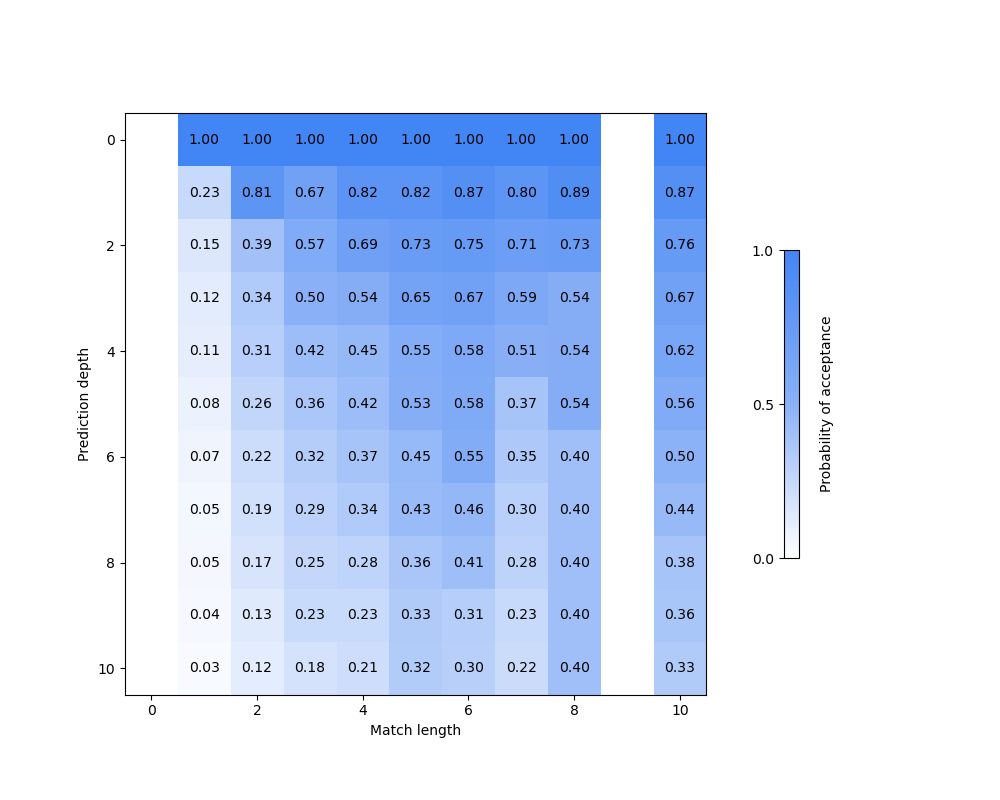
\includegraphics[width=.33\linewidth]{fig/prob_casd_accept.png} & 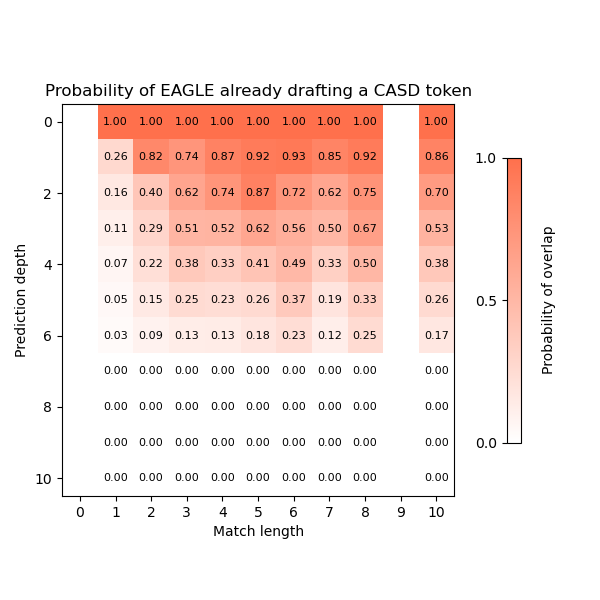
\includegraphics[width=.33\linewidth]{fig/prob_casd_eagle_overlap.png} & 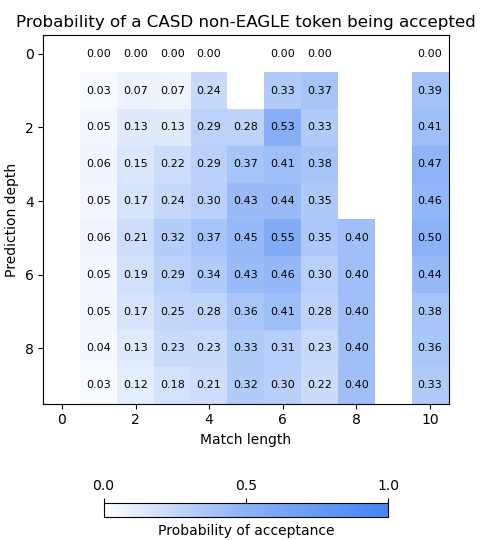
\includegraphics[width=.30\linewidth, height=.371\linewidth]{fig/prob_casd_non_eagle_accept.png} \\[0.5cm]
    \hspace{0.5cm} \parbox{.27\linewidth}{\small (a) CASD has long predictions of high quality, certainly for long match lengths. \newline \newline \newline} 
    & \hspace{0.5cm} \parbox{.27\linewidth}{\small (b) For few steps into the future, CASD's tokens often overlap with EAGLE-2, but tokens deeper into the future barely overlap. So, EAGLE-2 already has some notion of copying, but only for the near future.}
    & \hspace{0.5cm} \parbox{.27\linewidth}{\small (c) The tokens drafted by CASD and not by EAGLE-2 are accepted frequently, certainly for long match lengths. CASD gets most tokens accepted around depth 5, when augmenting EAGLE-2.} 
  \end{tabular}
  \vspace{0.2cm}
  \caption{
    Analysis of CASD's predictive power and its interaction with EAGLE-2.\\
    \textbf{Prediction depth:} how many steps in the future is the predicted token.\\
    \textbf{Match length:} number of tokens that correspond between the last generated tokens and the match in the context. \\
  }
  \label{fig:prob_casd_accept}
  \label{fig:prob_casd_eagle_overlap}
\end{figure}

\end{landscape}